In a Bayesian treatment of  hyper-parameter learning for \ac{GP}s,
we can write the probability of the hyper-parameters of a GP as
defined above, given covariance function $\mathbf{K}$ as:
\begin{equation}
\label{eq:hyperProbability}
P(\bm{\theta} \mid \mathbf{D,K}) = \frac{P(\mathbf{D} \mid \bm{\theta}, \mathbf{K})P(\bm{\theta} \mid  \mathbf{K})}{P(\mathbf{D} \mid \mathbf{K})}.
\end{equation}
Let $\mathbf{K}$ be the sum of a smoothing and a white noise (WN) kernel. For this case, Neal~\citeyearpar{neal1997monte} suggested the problem of outliers in data as a use-case for a hierarchical Bayesian treatment of Gaussian processes\footnote{In Neal's work \citeyearpar{neal1997monte} the sum of an SE plus a constant kernel is used. We keep the WN kernel for illustrative purposes.}. 
We can tackle this problem using \gpmem,
as illustrated with the tutorial in Fig. \ref{fig:neal_tutorial}. 
The main aim here is to  estimate the posterior of (\ref{eq:hyperProbability}) which we depict in panel (a) of Fig. \ref{fig:neal_tutorial}.

To arrive at this posterior, we must first have access to the data used in this problem. 
We define the data generating function as in Neal's paper. Let $f$ be the underlying function that generates the data:
\begin{equation}
f(x) =  0.3 + 0.4 x + 0.5 \sin(2.7x) + \frac{1.1}{(1+ x^2)} + \eta \;\;\; with\;\;\eta \sim \mathcal{N}(0,\sigma)
\end{equation}
We synthetically generate outliers by setting $\sigma = 0.1$ in $95\%$ of the cases and to $\sigma = 1$ in the remaining cases. 
This data set is accessed by a look-up function in Venture (Fig. \ref{fig:neal_tutorial} (b)).

\begin{figure}
\renewcommand{\arraystretch}{0.1}% Tighter
\centering \footnotesize
\begin{tikzpicture}
\node[] (start) {};
\node[left=1cm of start] (sfsigma) {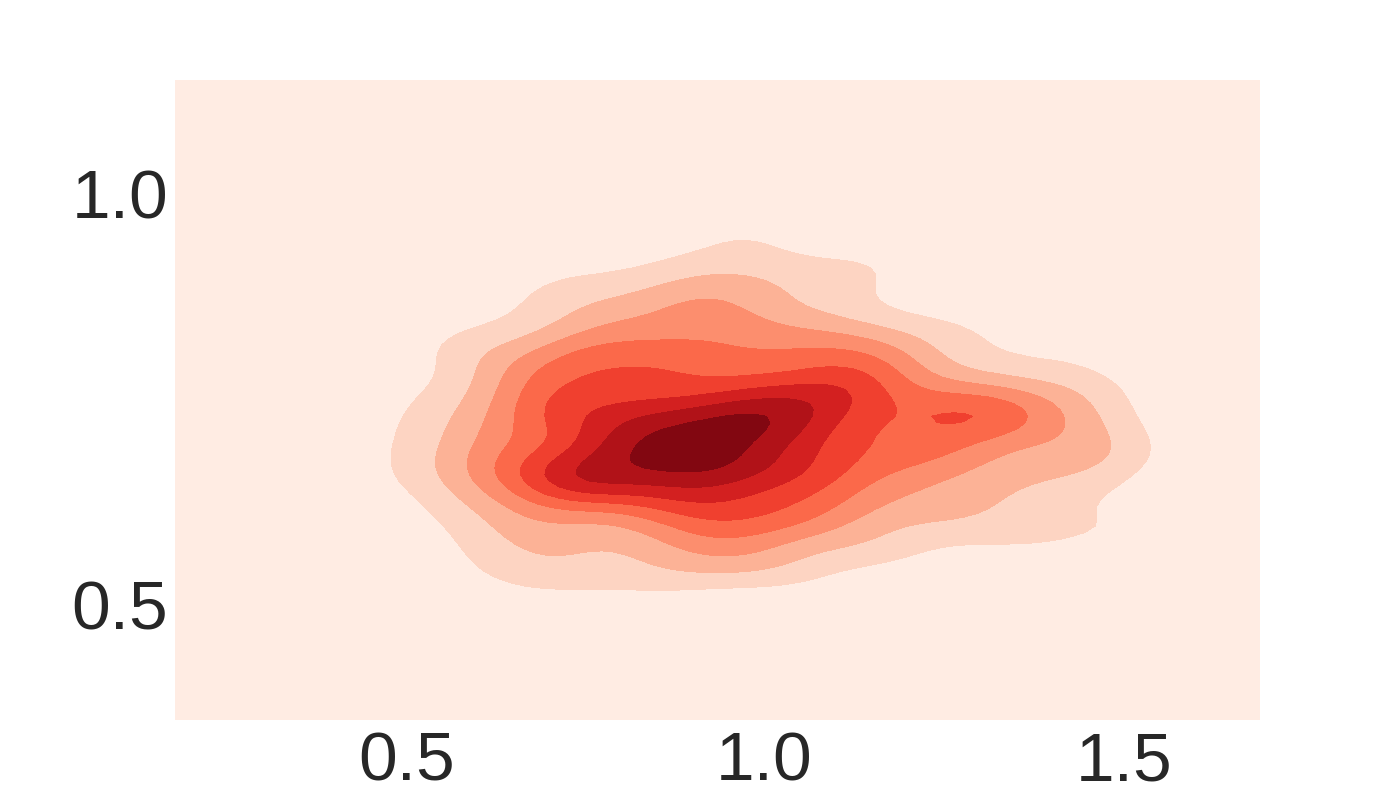
\includegraphics[height=2cm]{figs/hypers_sf_sigma.png}};
\node[right=1cm of start] (sfell) {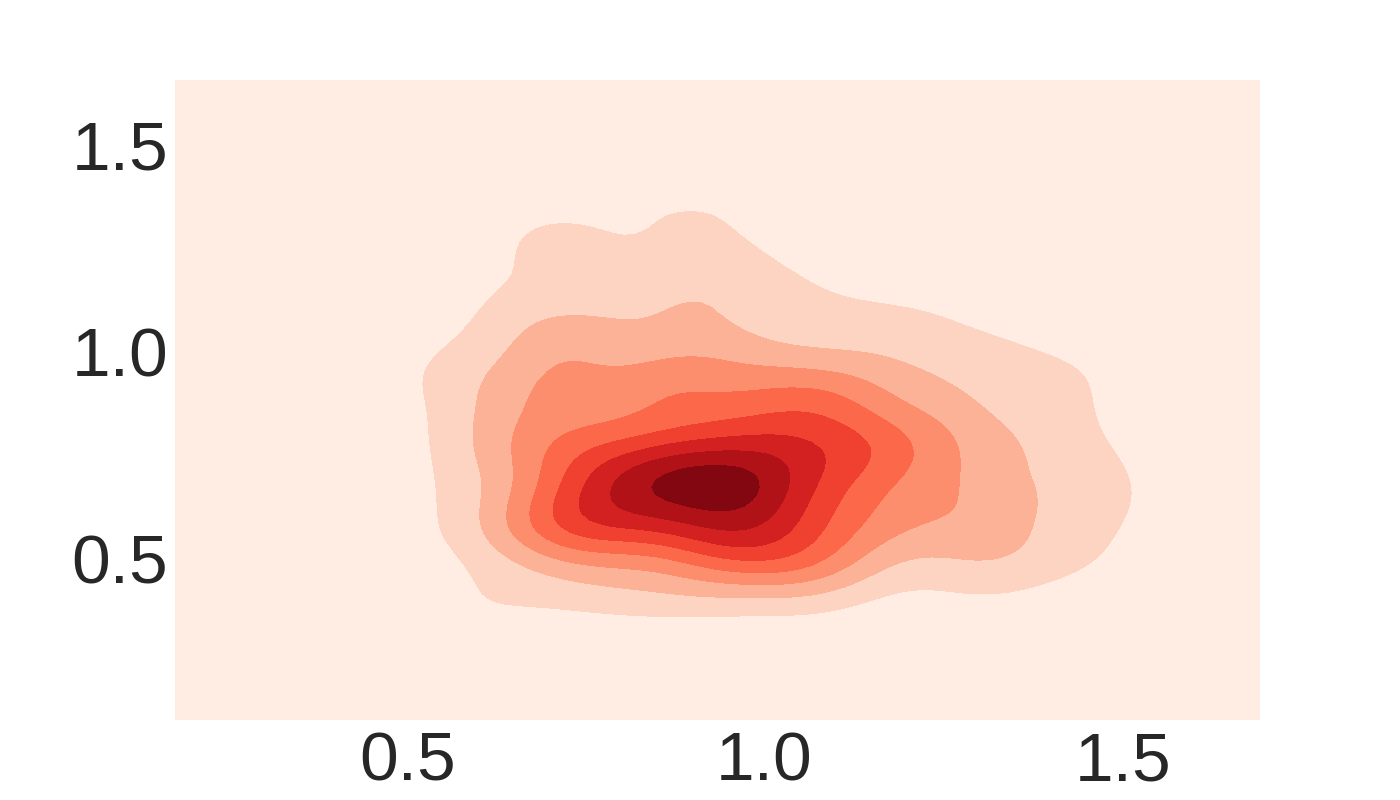
\includegraphics[height=2cm]{figs/hypers_sf_ell.png}};
\node[above=1cm of start] (hyper) {Hyper-Parameters for the Kernel:};
\node[left=0.cm of sfsigma] (ell) {$\ell$};
\node[below=0.cm of sfsigma] (sf1) {$sf$};
\node[left=0.cm of sfell] (sigma) {$\sigma$};
\node[below=0.cm of sfell] (sf2) {$sf$};
\end{tikzpicture}
\begin{tabular}{ll} \hline
\multicolumn{2}{}{}
  \begin{minipage}{4cm}
 \footnotesize\begin{lstlisting}
 // Data and look-up function
 define data = array(array(-1.87,0.13),..., array(1.67,0.81)) 
 assume f_look_up = proc(index) {lookup( data, index)}
\end{lstlisting}
\end{minipage}\\
\hline
\multicolumn{2}{}{}
  \begin{minipage}{4cm}
 \footnotesize\begin{lstlisting} 
 assume sf = tag(quote(hyper), 0, gamma(alpha_sf, beta_sf)))
 assume l = tag(quote(hyper), 1, gamma(alpha_l, beta_l)))
 assume sigma = tag(quote(hyper), 2, uniform_continuous(0, 2)) 
\end{lstlisting}
\end{minipage}
  \\
\hline
\footnotesize\begin{lstlisting}[ belowcaptionskip=0.1\baselineskip,mathescape,escapechar=\#]
// The covariance function
assume se = make_squaredexp(sf, l)
assume wn = make_whitenoise(sigma)
assume composite_covariance = add_funcs(se, wn)#\vspace{1mm}#
// Create a prober and emulator using gpmem
assume (f_compute, f_emu)
      = gpmem(f_look_up, composite_covariance)#\vspace{1mm}#
sample f_emu( array( -2, $\cdots$, 2)) 
\end{lstlisting}
 &  \raisebox{-0.5\height}{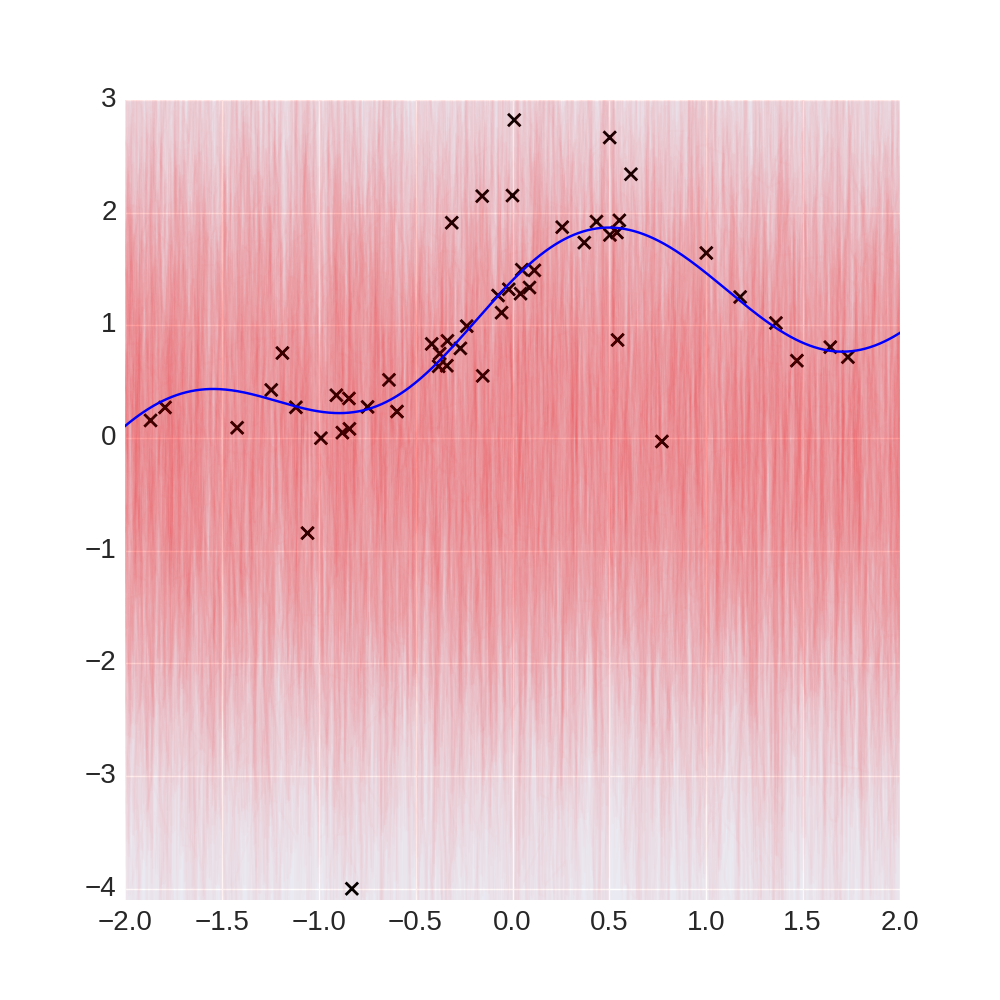
\includegraphics[height=3.4cm]{figs/neal_example_before_observation.png}}  \\ \hline
% line 3 

\footnotesize\begin{lstlisting}[aboveskip=-0.8 \baselineskip,mathescape,escapechar=\#]
// Observe all data points
for n ... N
    observe f_emu(first(lookup(data,n))) 
                = second(lookup(data,n))
// Or: probe all data points
for n ... N
    predict f_compute(first(lookup(data,n)))#\vspace{1mm}#
sample f_emu( array( -2, $\cdots$, 2)) 
\end{lstlisting}
 &  \raisebox{-0.5\height}{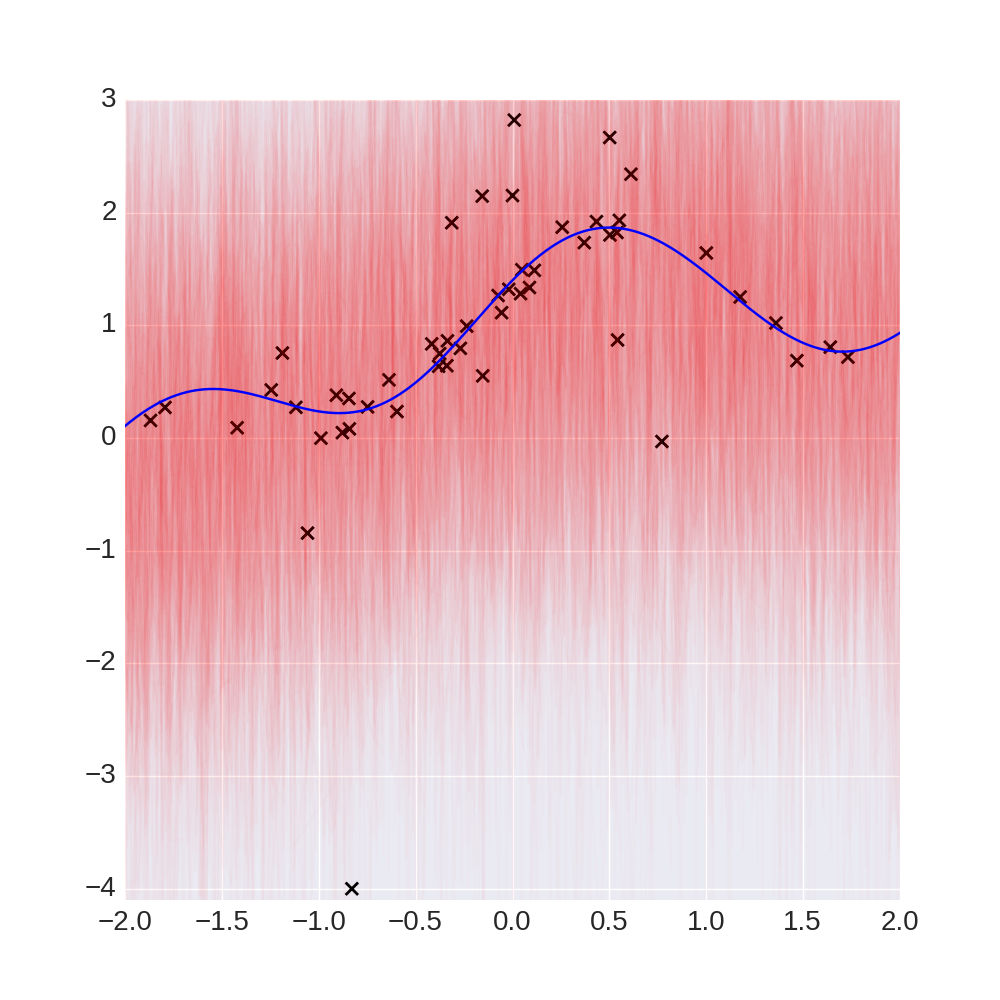
\includegraphics[height=3.4cm]{figs/neal_example_after_observation.png}}  \\ \hline
\footnotesize\begin{lstlisting}[mathescape,escapechar=\#]
// Metropolis-Hastings
infer repeat( 100, do(
                   mh( quote(hyperhyper), one, 2),
		   mh( quote(hyper),      one, 1)))#\vspace{1mm}#
sample f_emu( array( -2, $\cdots$, 2))   
\end{lstlisting}
 &   \raisebox{-0.5\height}{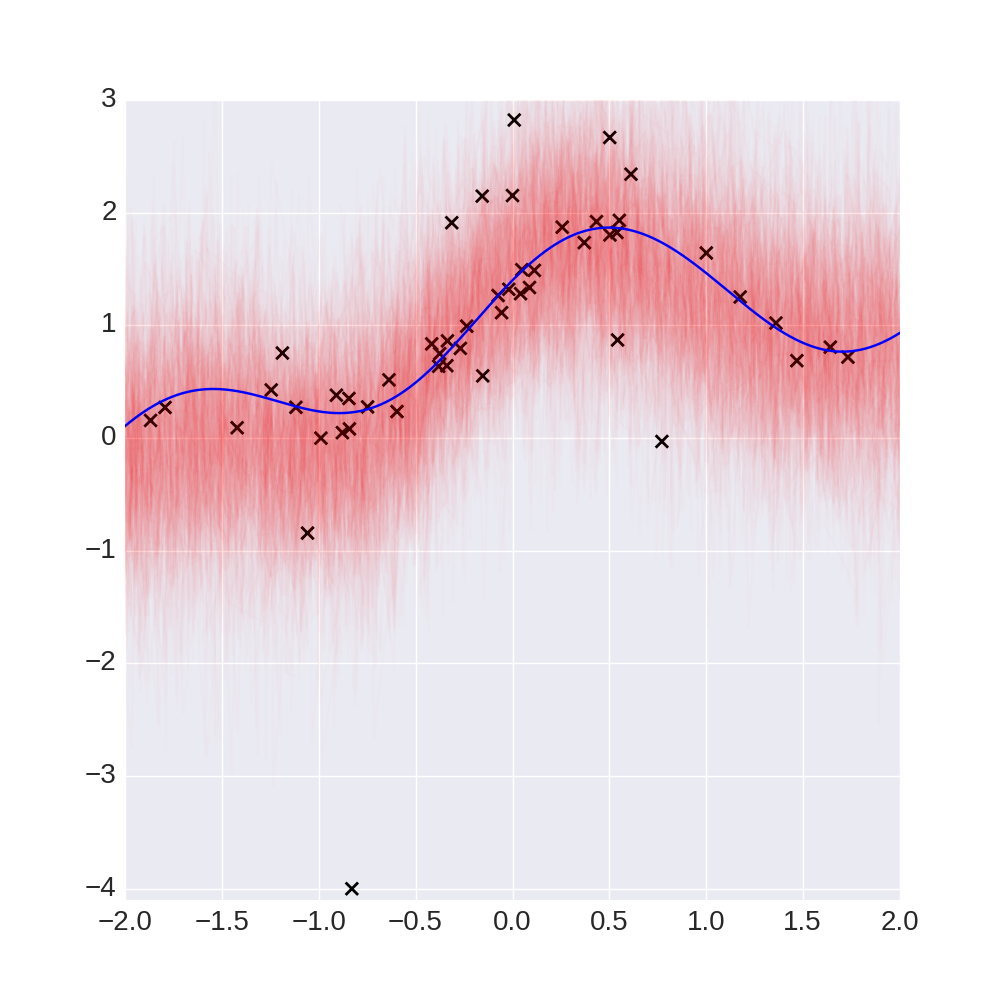
\includegraphics[height=3.4cm]{figs/neal_Bayesian.png}} \\ \hline
\footnotesize\begin{lstlisting}[mathescape,escapechar=\#]
// Optimization 
infer map( quote(hyper), all,0.01, 15)

sample f_emu( array( -2, $\cdots$, 2)) 
\end{lstlisting}
 &   \raisebox{-0.5\height}{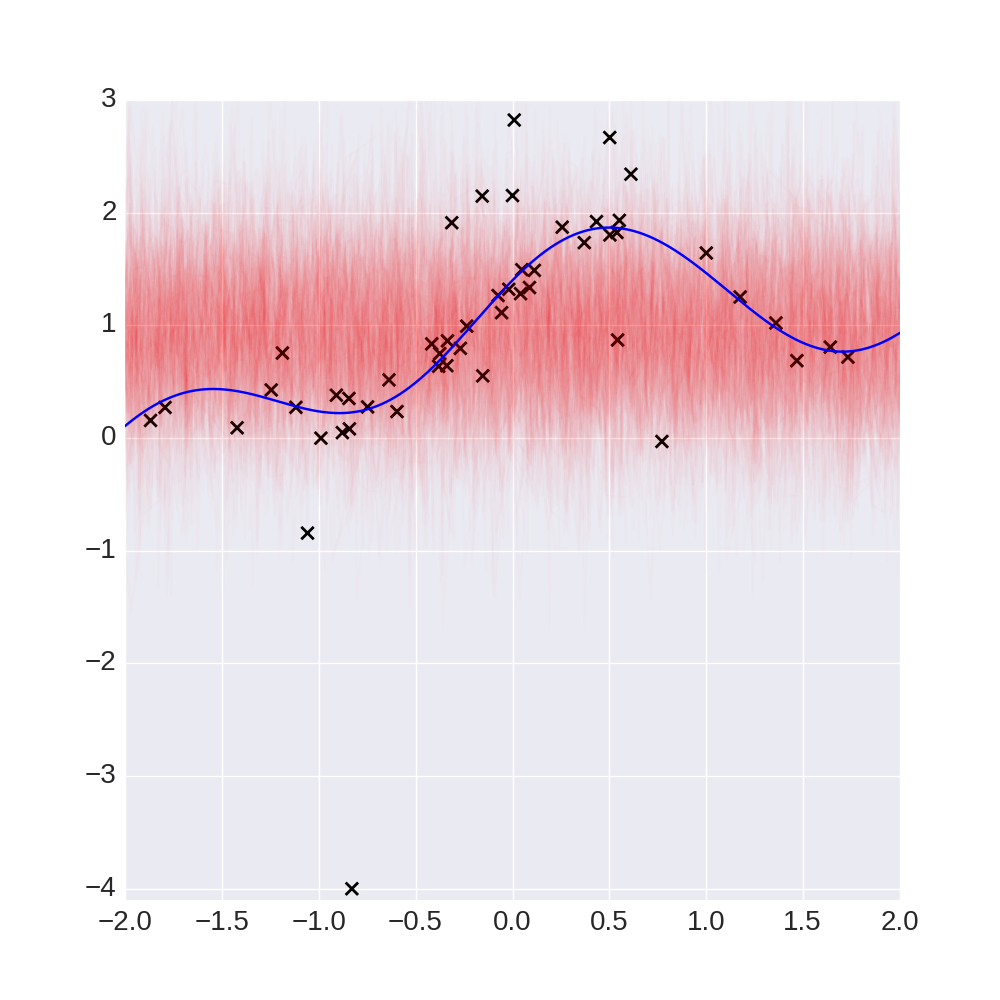
\includegraphics[height=3.4cm]{figs/neal_example_map_inference_alpha0p01_iter15.png}} \\ \hline
 
 \end{tabular}
\put(-410,230){(b)}
\put(-410,170){(c)}
\put(-410,90){(d)}
\put(-410,-10){(e)}
\put(-410,-110){(f)}
\put(-410,-210){(g)}
\caption{Regression with outliers and hierarchical prior structure}
\label{fig:neal_tutorial}
\end{figure}


Neals work suggests a hierarchical system of hyper-parameterization. Here, we draw hyper-parameters from $\Gamma$ distributions:
\begin{equation}
\label{eq:hyper-ell}
\ell^{(t)} \sim \Gamma(\alpha_1,\beta_1),\;\sigma^{(t)} \sim \Gamma(\alpha_2,\beta_2)
\end{equation} 
and in turn sample the $\alpha$ and $\beta$ from $\Gamma$ distributions as well:
\begin{equation}
\label{eq:hyper-alpha}
\alpha_1^{(t)} \sim \Gamma(\alpha^1_{\alpha},\beta^1_{ \alpha } ),\; \alpha_2^{(t)} \sim \Gamma(\alpha^2_{\alpha},\beta^2_{\alpha}),\cdots
\end{equation}
We model this in Venture as illustrated in Fig. \ref{fig:neal_tutorial} (c). Note that we omit the prior distributions of (\ref{eq:hyper-alpha}) due limited space in the tutorial.

In Fig. \ref{fig:neal_tutorial}, panel (c), we first construct a composite Kernel by adding a squared-exponential
covariance function to a white noise covariance function (SE and WN, Appendix A).
We then initialize \gpmem\ feeding it with the composite covariance and the data look-up function. 
We sample from the prior with random parameters $\texttt{sf,l}$ and $\texttt{sigma}$ and 
without any observations available.
We depict those samples on the right (red), alongside the true function that generated the data (blue) and
the data points we have available in the data set (black).

We can incorporate observations using both \texttt{observe} and \texttt{predict} (Fig. \ref{fig:neal_tutorial} (e)).
When we subsequently sample from the emulator, we can now see that the \ac{GP} posterior incorporates knowledge 
about the data points. Yet, the hyper-parameters are still random, so the emulator does not capture the true
underlying dynamics of the data correctly. 

Next, we demonstrate how we can capture these underlying dynamics within only 100 \ac{MH} steps on the hyper-parameters to get a good approximation for their posterior (Fig. \ref{fig:neal_tutorial} (f)).
Note that Neal devises an additional noise model and performs a large number of Hybrid-Monte Carlo and Gibbs steps to achieve this, whereas inference in Venture with \gpmem\ is merely one line of code. 

Finally, we can change our inference strategy altogether. If we decide that instead of following a Bayesian sampling approach,
we would like to perform empirical optimization, we do this by only changing one line of code (Fig. \ref{fig:neal_tutorial} (g)). 

